\documentclass[a4paper,12pt]{article}
\usepackage{graphicx}
\usepackage{tikz}
\usepackage{setspace}
\usepackage[margin=1in]{geometry}
\usepackage{url}
\begin{document}

\begin{titlepage}
\begin{center}
\vspace*{4cm}

\hrule
\vspace{0.4cm} 
{\LARGE \bfseries Graphs with Identical }\\[1mm]
{\LARGE \bfseries Chromatic Symmetric Functions}\\[0.4cm]
\hrule
\vspace{1.2cm}

\textsc{\Large A Proposal for the}\\[0.2cm]
\textsc{\Large Undergraduate Research Award}\\[2cm]

\begin{minipage}{0.4\textwidth}
\begin{flushleft} \large
\hspace{1cm}\emph{Author:}\\
Keeler M. Russell
\end{flushleft}
\end{minipage}
\begin{minipage}{0.4\textwidth}
\begin{flushright} \large
\emph{Mentor:}\ \ \ \ \ \ \ \ \ \ \ \\
Dr. Jeremy L. Martin
\end{flushright}
\end{minipage}
\vspace{3cm}

\vfill
\includegraphics[scale=0.15]{./figures/kujayhawk.png}\\
\textsc{University of Kansas}\\[0.75cm]
{\large \today}
\end{center}
\end{titlepage}

\begin{spacing}{1}

\section*{\Large Project Description}
\hrule
\vspace{0.4cm}
\subsection*{Summary of Purpose}
All graphs, sets of vertices joined by edges, have an associated chromatic symmetric function $X_G$. This project focuses on whether or not a tree, a particular type of graph, can be reconstructed uniquely from its chromatic symmetric function. This is an open, or unanswered, question in mathematics, defined more fully throughout the course of this proposal.

\subsection*{Background Information}
A \emph{graph} $G$, denoted $G(V, E)$, is a set of vertices $V$ connected by a set of edges $E$. A \emph{tree} $T$ is a graph such that any two vertices are connected by a unique \emph{simple path}, a sequence of distinct vertices such that each vertex is connected to the next in the sequence by a single edge. An excellent entry-level introduction to graph theory is \cite{walkthroughcombinatorics}.

We say that two graphs are \emph{isomorphic} if they are structurally identical.  Also, an \emph{invariant} is a property of a graph $G$ that depends only on the structure of $G$, and not on a particular representation or drawing of $G$. For example, the number of vertices in a graph or number of edges in a graph are simple invariants. Isomorphic graphs, since they are structurally identical, must have the same values for their invariants. However, note that the reverse is not true in general: two non-isomorphic graphs can have the same values for invariants. For example, consider Figure 1: both graphs have the same number of vertices and edges, yet they are distinct structurally. A \emph{complete invariant} is one that is unique to an isomorphic graph; that is, only that graph and no others can have that value for the invariant, thus enabling reconstruction of that graph from its invariant.

A \emph{proper coloring} is an assignment of colors to the vertices of a graph such that no two adjacent vertices (vertices which share an edge) share a color. It has been shown, by modelling it as a graph coloring problem, that at most 4 colors are required to color the territories on a map such that no adjacent territories have the same color \cite{fourcolor1, fourcolor2}. This is arguably the most famous problem in the history of graph theory. In computer science, graph coloring is used in process scheduling: a different vertex represents each process, and an edge connects two processes if they cannot execute concurrently. The chromatic number of this graph gives the minimum number of cycles needed to execute these processes. Coloring problems are computationally difficult in general.

The \emph{chromatic polynomial} $\chi_G(k)$ counts the number of proper colorings of $G$ given at most $k$ colors. This is another type of invariant. For any tree $T$, $\chi_T(k) = k(k - 1)^{n - 1}$, where $n$ is the number of vertices in the tree \cite{bollobasgraphs}. The chromatic polynomial does not distinguish trees because it gives the same information regardless of the structure of the tree.

Symmetric functions can be used to encode more information about a graph's proper colorings. A symmetric function is any power series in infinitely many variables $x_i$ that doesn't change if its variables are interchanged \cite{enumerative}. Building on the chromatic polynomial, Richard Stanley introduced another invariant, the \emph{chromatic symmetric function}~$X_G$, as a symmetric function generalization of the chromatic polynomial \cite{csfstanley}. The chromatic symmetric function $X_G$ of a graph $G$ is a function which counts, for each way to write~$n$ as the sum of positive integers $\lambda_1, \lambda_2, \lambda_3, \ldots$, the number of proper colorings using color~$i$~$\lambda_i$ times. Each term in the chromatic symmetric function represents a proper coloring, where the exponent of each variable $x_i$ indicates the number of times to use color $i$. Permuting the names of the colors does not affect whether the coloring is proper, which is why this function is symmetric. For example, in Figure 1, the term $4m_{2,2,1}$ in $X_G$ indicates that there are 4 distinct ways to color two vertices one color, two other vertices a second color, and one final vertex a third color.

Here, we may state the overall research question concretely: is $X_T$ a complete isomorphism invariant for trees? That is, does $X_T$ determine a tree's structure up to isomorphism? Or, equivalently, can any two non-isomorphic trees to have the same $X_T$?

Firstly, it \emph{is} possible for two distinct graphs to have the same chromatic symmetric function, so it is not a complete isomorphism invariant for graphs in general (see Figure 1) \cite{csfstanley}. However, it is unknown whether $X_T$ is a complete isomorphism invariant for trees, which is the question this research aims to tackle. For trees with 23 or fewer vertices, in his undergraduate thesis Li-Yang Tan showed through exhaustive computation that no trees of 23 vertices or less have the same~$X_T$ \cite{tantrees}.

Additionally, Martin, Morin, and Wagner \cite{distinguishtrees} have shown that certain important invariants can be recovered from the chromatic symmetric function of trees and that for certain classes of trees, $X_T$ distinguishes them up to isomorphism. This is the state of the art for the chromatic symmetric function.

\begin{figure}[t]
\begin{center}
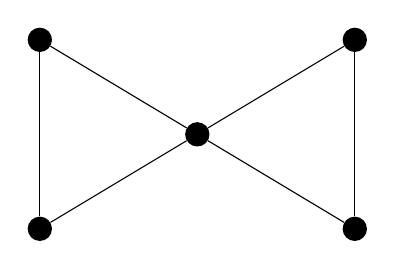
\begin{tikzpicture}
  [scale=.4,auto=left,every node/.style={circle,fill=black,scale=0.5}]
  \node (n1) at (0,0)  {1};
  \node (n2) at (0,6)  {2};
  \node (n3) at (5,3)  {3};
  \node (n4) at (10,6)  {4};
  \node (n5) at (10,0)  {5};

  \foreach \from/\to in {n1/n2,n1/n3,n2/n3,n3/n4,n3/n5,n4/n5}
    \draw (\from) -- (\to);
\end{tikzpicture}
\hspace{1cm}
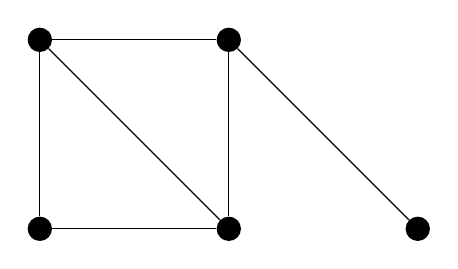
\begin{tikzpicture}
  [scale=.4,auto=left,every node/.style={circle,fill=black,scale=0.5}]
  \node (n1) at (0,0)  {1};
  \node (n2) at (0,6)  {2};
  \node (n3) at (6,6)  {3};
  \node (n4) at (6,0)  {4};
  \node (n5) at (12,0)  {5};

  \foreach \from/\to in {n1/n2,n1/n4,n2/n3,n2/n4,n3/n4,n3/n5}
    \draw (\from) -- (\to);
\end{tikzpicture}
\caption{Two graphs $G$ and $H$ with the same chromatic symmetric function. In this case, $X_G = X_H = 120m_{1,1,1,1,1} + 24m_{2,1,1,1} + 4m_{2,2,1}$.}
\end{center}
\end{figure}

\subsection*{Aim of Research}
The first goal is computationally determine whether trees of greater than 23 vertices have the same $X_T$. The reference to Tan's work \cite{tantrees} is now unstable (although I do have a copy of his source code through personal communication), and by reproducing and potentially improving on his results I will provide a stable, open-source reference to my work. If this is accomplished, a pair of trees forming a counterexample for the open question given above may be found, and this pair can be analyzed to determine exactly \emph{why} they each have different $X_T$. If such a counterexample is not found, then at the very least the boundary of 23 vertices will have been breached, and the code that I will write for these computations can be made freely available online for future research.

The second goal is purely mathematical: to construct an infinite family of pairs of graphs $(G_0, H_0),\ (G_1, H_1),\ (G_2, H_2),\ \ldots$ for which $X(G_i)$ is identical to $X(H_i)$ for all natural numbers $i$. Stanley, in his original paper introducing $X_G$, presented a pair of graphs which have the same $X_G$, one which looks like a bow tie, the other something like a kite (see Figure 1). By `gluing' copies of these graphs together in a clever way, a method could be provided for constructing an infinite number of graphs with the same chromatic symmetric function. This resembles Gordon and Eisenstat's construction of an infinite family of non-isomorphic `caterpillar' trees with identical subtree data \cite{caterpillarfamily}. Although it would not answer the open question for trees, it would represent an opposing line of inquiry which examines \emph{why} this infinite family has pairs of graphs with the same $X_G$. This could provide insight into what sort of qualities make one graph's $X_G$ differ from another's.

The third, most abstract, and most difficult goal is to treat the chromatic symmetric function as a linear transformation from the vector space of graphs to the vector space of symmetric functions. This transformation must have a non-trivial \emph{kernel} or \emph{nullspace}, a set that contains the linear combinations of graphs that map to 0, since the dimension of the vector space of graphs with $n$ vertices is much larger than the dimension of the vector space of symmetric functions of degree $n$. The key is to determine what kinds of linear combinations exist in the kernel. Given two graphs $G$ and $H$ with the same number of vertices, if $X_G = X_H$ then the formal linear combination $G - H$ is in the kernel. By understanding the kernel of this transformation, it may be possible to gain new insight into the open question of the chromatic symmetric functions of trees. Note that if the linear combination of trees $T-U$ can be found in the kernel, then $T$ and $U$ share the same chromatic symmetric function, thus answering Stanley's question.

\subsection*{Methods}
The first step is to develop a program that generates all non-isomorphic trees on $n$ vertices, then check to make sure that none of them have the same chromatic symmetric function. My primary tool in this investigation will be \emph{Sage}, an open-source mathematics software package \cite{sagemath}. I have already written Sage code which correctly computes the chromatic symmetric function of a graph, and am now working on speeding this code up. It is worth noting that for graphs in general, the isomorphism problem becomes infeasible: the number of graphs on $n$ vertices grows exponentially, and a fast algorithm for this isomorphism-checking process is not known. However, for trees, there exist efficient algorithms for enumerating all trees on $n$ vertices \cite{generatefreetrees} and for checking for isomorphism between two trees \cite{Buss97alogtimealgorithms}, though I have not found any Sage implementation of these algorithms, so I may have to implement them myself.

Constructing an infinite family of non-tree graphs with identical $X_T$ involves more intuition than programming. Dr. Martin has confirmed this goal's feasibility. I can investigate Stanley's original paper on the chromatic symmetric function further for insight into this problem. Additionally, Martin, Morin, and Wagner's work in \cite{distinguishtrees} serves as a reference for the combinatorial interpretation of the coefficients of $X_G$. With some effort and fact-checking using Sage, I should be able to construct such a family.

The third and final goal will require additional education and work on my part. In order to tackle it, I will need to expand my knowledge of linear algebra. In the process of completing the first and second goals of this project, I am confident that I will pick up enough intuition about the chromatic symmetric function to make a reasonable stab at this problem. It is a more generalized version of the second goal, and so the same methods as above will apply.

\subsection*{Scientific Significance}
The Sage code I will write will push the frontier of what is known about the chromatic symmetric function of a tree beyond the current state of the art, potentially discerning an answer to Stanley's open question of whether $X_T$ is a complete isomorphism invariant for trees. I will also provide a stable reference to my code, since Tan's code is no longer freely available online. Additionally, my code will be of use to other researchers in attacking chromatic symmetric function research in general, a much researched topic in mathematics. For example, research on the \emph{3+1 conjecture}, introduced by Stanley in \cite{csfstanley} can benefit from the code I will write.

\section*{\Large Personal Significance}
\hrule
\vspace{0.4cm}
First and foremost, this project is exciting for me. I plan on continuing my education by acquiring a masters degree, with Computer Science and Mathematics as my two primary choices. I consider this project an excellent preparation for graduate study, allowing me to try pushing against the limits of human knowledge in these fields simultaneously before even reaching graduate school.

I plan to publish my research in an appropriate journal, such as the Rose-Hulman Undergraduate Mathematics Journal \cite{rosehulman} or the Journal of Young Investigators \cite{jyi}. I also plan to present at a conference. Many mathematics conferences encourage presentations by students, for example the Joint Mathematics Meetings in San Diego, CA during January 2013, the major professional mathematics conference. If I planned to present at this conference, that would allow me a little less than a year to conduct my investigation. I would also like to present at the KU Honors Symposium in Fall 2012.

\section*{\Large My Qualifications}
\hrule
\vspace{0.4cm}
This proposal requires knowledge of computing techniques to develop a correct and efficient algorithm for generating trees and checking their chromatic symmetric functions against one another. I feel that I am up to the task for several reasons: for one, I am a Computer Engineering student, and have formal training in algorithm development and analysis. Secondly, I make a living as a programmer working for Garmin on embedded GPS device code, meaning that I have programmed nearly every day for several years. Finally, I was awarded the Eta Kappa Nu Underclassman Achievement Award for being the top student in Programming II.

Additionally, during the summer of 2010, just after my freshman semester, I participated in the Honors Research Development Program, drafting a proposal with Dr. Martin. My current proposal is based on the work I completed during that summer, which included reading research papers, learning elementary graph theory, and drafting academic papers using \LaTeX. During the interim since then, I have completed more mathematics and computer science courses, such as Elementary Linear Algebra (MATH 290), Software Engineering (EECS 443), and Programming II (EECS 268) in particular, which make me prepared to tackle a research project like this. I also plan on taking Algorithms and Data Structures (EECS 560) and Linear Algebra (MATH 590), which will also help. With my greater understanding of the tasks at hand, I feel strongly qualified for this project and this research award.

\end{spacing}

\pagebreak
\bibliographystyle{plain}
\bibliography{references}
\end{document}